

%caso 1
\subsection{Autenticação de bebidas}
Este caso consiste da implementação de um sistema RFID pela fabricante de bebidas de Taiwan \textit{Taiwan Tobacco and Liquor Corp.} (TTL). O objetivo da adoção foi assegurar a autenticidade de seus produtos e rastrear as mercadorias pela cadeia de suprimentos. 
A empresa produz principalmente vinhos finos e bebidas de alto valor, portanto é de seu interesse garantir a autenticidade de seus produtos, principalmente no mercado da China.

Para desenvolver este sistema, a TTL decidiu trabalhar com a EPC Solutions Taiwan. A solução deveria ser capaz de todos os produtos em sua cadeia de suprimentos, passando pelo engarrafamento, embalagem e recebimento de mercadorias no centro de distruibuição (CD) na China.  Além disso, os clientes deveriam ser capazes de confirmar a autenticidade do produto através de um leitor portátil, o qual interrogaria o rótulo de cada garrafa.

Como a TTL deveria fornecer um leitor para cada revendedor, a escolha deste era um fator crucial projeto, pois era preciso um leitor que funcionasse bem e barato. Para isso, A EPC Solutions desenvolveu um leitor de baixo custo operando em 433 MHz capaz de ler as tags RFID passivas EPC Gen2 UHF escolhidas para a aplicação. 

\begin{figure}[h!]
\centering
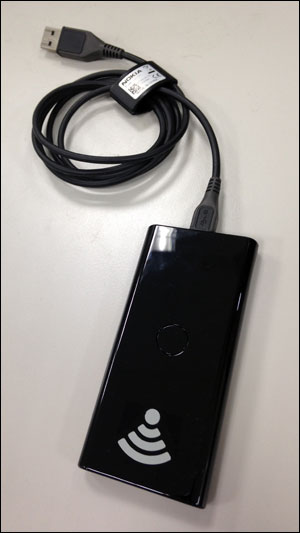
\includegraphics[width=0.2\linewidth]{leitor_ttl}
\caption{Leitor desenvolvido}
\label{fig:leitor_ttl}
\end{figure}
   
Nos armazéns, fábricas e centros de distribuição, foram instalados três leitores UHF 902-928 MHz para interrogar as tags. Escolheu-se um frequência de operação maior de forma a permitir a leitura a maiores distâncias.

Na estação de engarrafamentoe, as tags são afixadas no topo da garrafa através de um adesivo não removível, interrogadas automaticamente e seus dados são enviados a servidor back-end da TTL, onde o software relaciona o tipo de produto e lote com o número de identificação único da tag.

Ao chegar na estação de embalagem, os funcionários empacotam 6 garrafas em uma caixa e adicionam outra tag à esta caixa. Todas a 7 tags são lidas pelo próximo interrogador, o qual vincula as tags dos frascos à da embalagem.

Por fim, as caixas são carregadas em paletes e um leitor fixos lê as tags das garrafas e da caixa, relacionando essa informação com a etiqueta afixada no palete. Os paletes são então transferidos para o armazém, onde leitores fixos registram a chegada dos bens e funcionários com leitores de mão fazem verificações periódicas de inventário.

No momento da expedição, os bens passam por um portal leitor fixo que atualiza o software e indica que o palete foi enviado ao CD. No CD, leitores fixos foram instalados para indicar o recebimento do palete e equipamentos de mão são usados para controle de estoque. Os dados são então enviados ao servidor da TTL para atualização.

Nas lojas, os consumidores podem conectar o leitor \ref{fig:leitor_ttl} ao seu tablet ou smartphone e baixar o aplicativo da TTL para conseguir confirmar a autenticidade do produt através da leitura da tag do produto. Em cada leitura, um consulta é feita ao servidor da TTL, de forma a garantir esta procedência.


%caso 2
\subsection{Melhora no Workflow de Hospital}
Em 2013, o diretor de serviços de informação do departamento de engenharia biomédica do University Hospital (da University Health System em San Antonio, Texas) encontrou um grave problema no hospital onde trabalha: enfermeiros estavam escondendo bombas IV por serem muito escassas neste hospital e para terem disponível quando um paciente precisasse.

Esse diretor e um gerente de tecnologias de cuidados da saúde do hospital decidiram implantar um sistema para rastrear as bombas IV e outros equipamentos e assim acabar com o monopólio dos mesmos. 

Em março de 2014, um sistema de localização em tempo real baseado em RFID passiva ja havia sido implementado nas instalações do hospital. Assim foi possível controlar e gerenciar todas bombas médicas do hospital. Como resultado a taxa de uso dessas bombas médicas inteligentes passaram de menos de 45\% por cento para mais de 70\%.

Para esse projeto foram usados tags Confidex Steelwave Micro RFID UHF e colocados nas bombas. Os leitores fixos de RFID Zebra Technologies FX7500 foram instalados nas salas onde as bombas são devolvidas após o uso. Nas salas também foram instaladas as antenas Five-foot-long Wave da NeWave Sensor Solutions e Advantenna-p33 da Keonn Technologies.

A taxa e leitura das tags deveria ser próxima de 100\%. Foi feito um teste de campo para validar a escolha de hardware e os leitores e antenas foram instalados nas salas localizadas em cada unidade de internação. Os leitores também foram instalados nos centros de distribuição de equipamentos central do hospital e o departamento de engenharia biomédica para acompanhar o uso, manutenção e armazenamento dos equipamentos. Além das bombas IV, o hospital passou a rastrear bombas de alimentação, drenos, bombas de grande volume e bombas de analgesia controladas pelo paciente.

O hospital ainda implantou uma plataforma de software para controlar e gerenciar bombas e automatizar os processos de fluxo de trabalho com RFID. Com o novo sistema, encerrou-se o monopolio dos equipamentos. Antes, quando uma enfermeira necessitava de uma bomba ela poderia ter que esperar por duas horas para receber o equipamento. Agora, com esse sistema, o tempo de espera médio fica em torno de 6 a 8 minutos.

